\documentclass[tikz,border=15pt]{standalone}
\usepackage{tikz}
\usetikzlibrary{shapes.geometric, arrows.meta, positioning}

\tikzset{
    register/.style={
        rectangle, draw=black, thick,
        minimum width=1.8cm, minimum height=1.1cm,
        fill=white, font=\small\ttfamily
    },
    mux/.style={
        trapezium, trapezium left angle=70, trapezium right angle=110,
        draw=black, thick,
        minimum width=1.1cm, minimum height=0.95cm,
        fill=white, font=\small
    },
    alu/.style={
        rectangle, draw=black, thick,
        minimum width=1.3cm, minimum height=1.1cm,
        fill=white, font=\small
    },
    wire/.style={draw=black, thick, -Stealth},
    bus/.style={draw=black, line width=1.8pt, -Stealth},
    controlwire/.style={draw=black!60, dashed, -Stealth},
    buswidth/.style={font=\scriptsize, fill=white, inner sep=2pt},
    logic/.style={
        rectangle, draw=black, thick, rounded corners=3pt,
        minimum width=1.1cm, minimum height=1cm,
        fill=gray!10, font=\small
    },
    sbox/.style={
        rectangle, draw=black, thick,
        minimum width=0.95cm, minimum height=0.95cm,
        fill=gray!20, font=\small
    }
}

\begin{document}
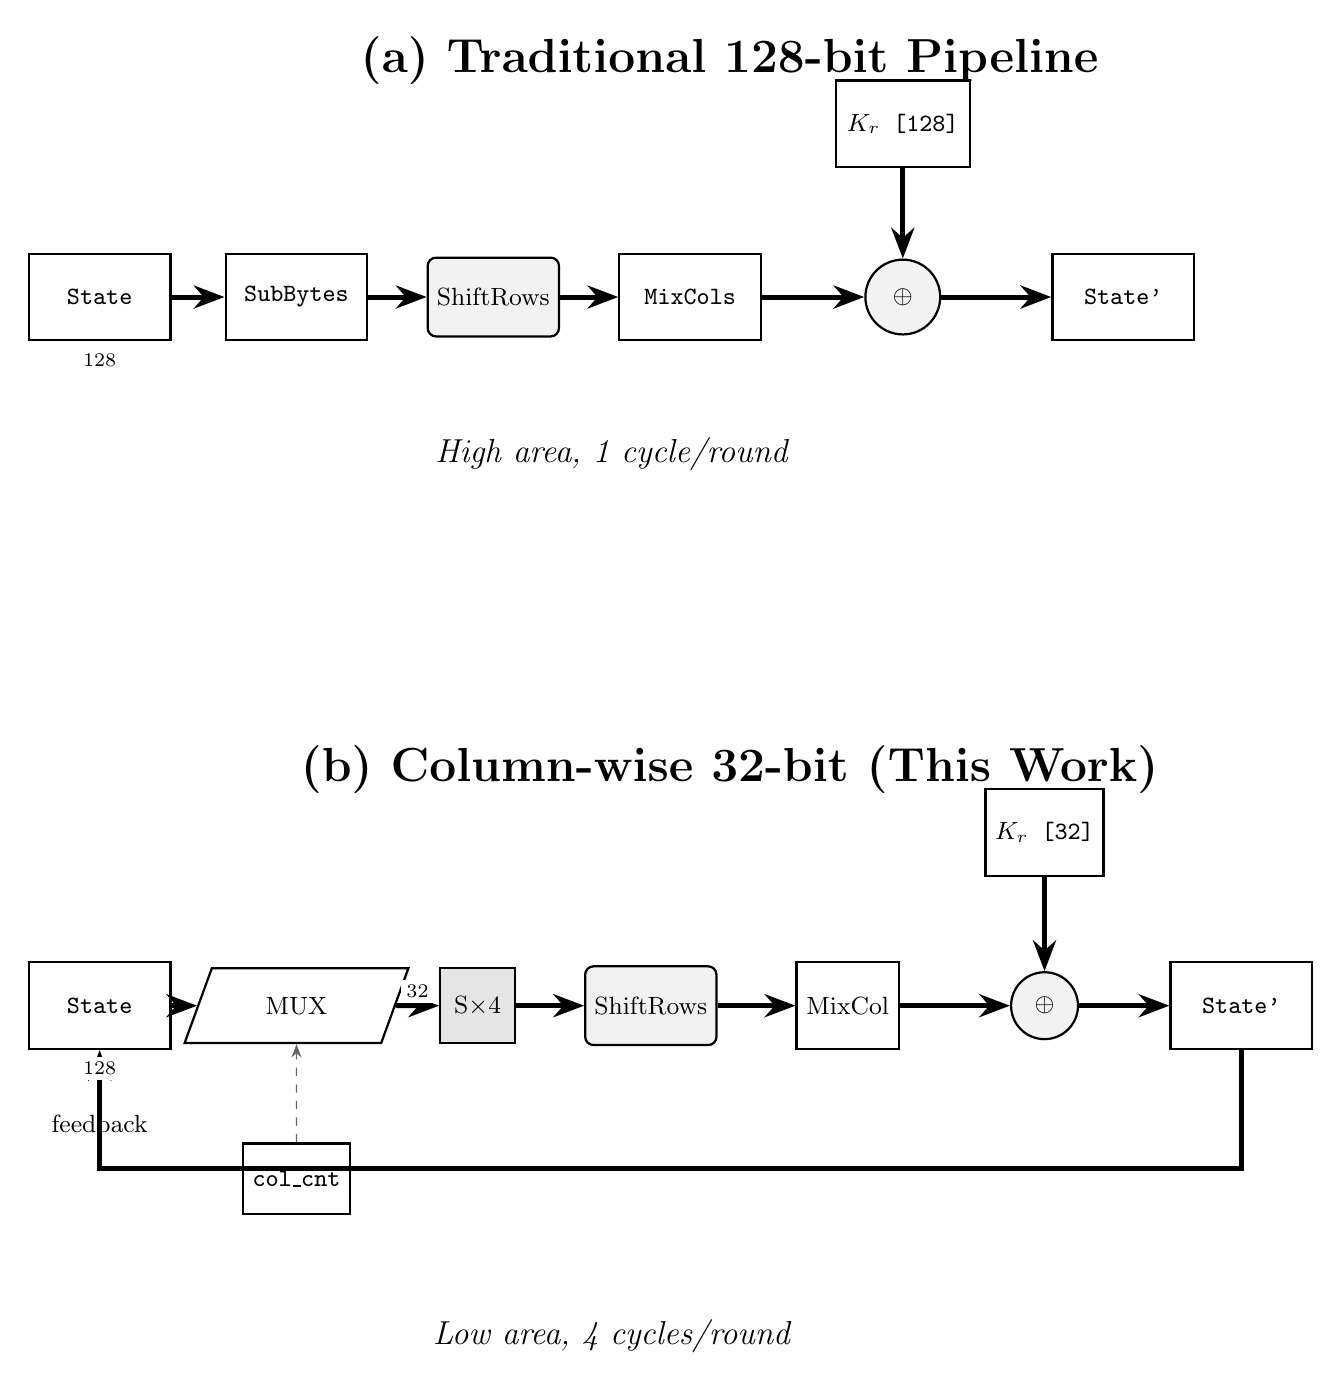
\begin{tikzpicture}

% (a) Traditional 128-bit Pipeline
\node[font=\LARGE\bfseries] at (8,5) {(a) Traditional 128-bit Pipeline};

\node[register] (s0) at (0,2) {State};
\node[register] (sb) at (2.5,2) {SubBytes};
\node[logic] (sr) at (5,2) {ShiftRows};
\node[register] (mc) at (7.5,2) {MixCols};
\node[logic, circle, minimum size=0.95cm] (xor) at (10.2,2) {$\oplus$};
\node[register] (s1) at (13,2) {State'};

\node[register, minimum width=1.7cm] (rk) at (10.2,4.2) {$K_r$ [128]};

\draw[bus] (s0) -- (sb);
\draw[bus] (sb) -- (sr);
\draw[bus] (sr) -- (mc);
\draw[bus] (mc) -- (xor);
\draw[bus] (xor) -- (s1);
\draw[bus] (rk) -- (xor);

\node[buswidth] at (0,1.2) {128};
\node[font=\large\itshape] at (6.5,0) {High area, 1 cycle/round};

% (b) Column-wise 32-bit Pipeline
\node[font=\LARGE\bfseries] at (8,-4) {(b) Column-wise 32-bit (This Work)};

\node[register] (t0) at (0,-7) {State};
\node[mux] (tmux) at (2.5,-7) {MUX};
\node[sbox] (tsb) at (4.8,-7) {S$\times$4};
\node[logic, minimum width=1.6cm] (tsr) at (7,-7) {ShiftRows};
\node[alu] (tmc) at (9.5,-7) {MixCol};
\node[logic, circle, minimum size=0.85cm] (txor) at (12,-7) {$\oplus$};
\node[register] (t1) at (14.5,-7) {State'};

\node[register, minimum width=1.5cm] (trk) at (12,-4.8) {$K_r$ [32]};
\node[register, minimum width=1.3cm, minimum height=0.9cm] (cnt) at (2.5,-9.2) {col\_cnt};

\draw[bus] (t0) -- (tmux);
\draw[bus] (tmux) -- node[buswidth, above] {32} (tsb);
\draw[bus] (tsb) -- (tsr);
\draw[bus] (tsr) -- (tmc);
\draw[bus] (tmc) -- (txor);
\draw[bus] (txor) -- (t1);
\draw[bus] (trk) -- (txor);

% Feedback path - routed well below
\draw[bus] (t1.south) -- ++(0,-1.5) -| node[pos=0.6, above, font=\small] {feedback} (t0.south);

\draw[controlwire] (cnt) -- (tmux);

\node[buswidth] at (0,-7.8) {128};
\node[font=\large\itshape] at (6.5,-11.2) {Low area, 4 cycles/round};

\end{tikzpicture}
\end{document}
